\chapter{Discussion}
We have learned from our data set and its features that they are a viable candidate for machine learning purposes and this course through different visualizations of deviation, correlation and PCA on the attributes. 

We do not have very meaningful attributes when they stand by themselves, i.e. the amount of pixels in the third row is pretty unimportant negligible. However, together the attributes compliment each other well and makes it very possible to see good correlation within the classes as well as being able to distinguish them and their digits apart.

The data set has also shown to be quite viable for further analysis and for applying various machine learning techniques. We can already see ways of being able to classify most of the numbers with good reliability, and doing further modelling will only help in this regard.

It should also be noted that the data have been projected on to the PCs and plotted with scatter plots, but to comply with the ACCENT principles the projections have been visualized as in Figure~\ref{fig:pca_projections_explained} for easier interpretation and at the end we modified the scatter plot such it draws the numbers instead of dots and the result can be seen in Figure~\ref{fig:pc_projections} to be interpreted. 

\begin{figure}[hbtp]
\centering
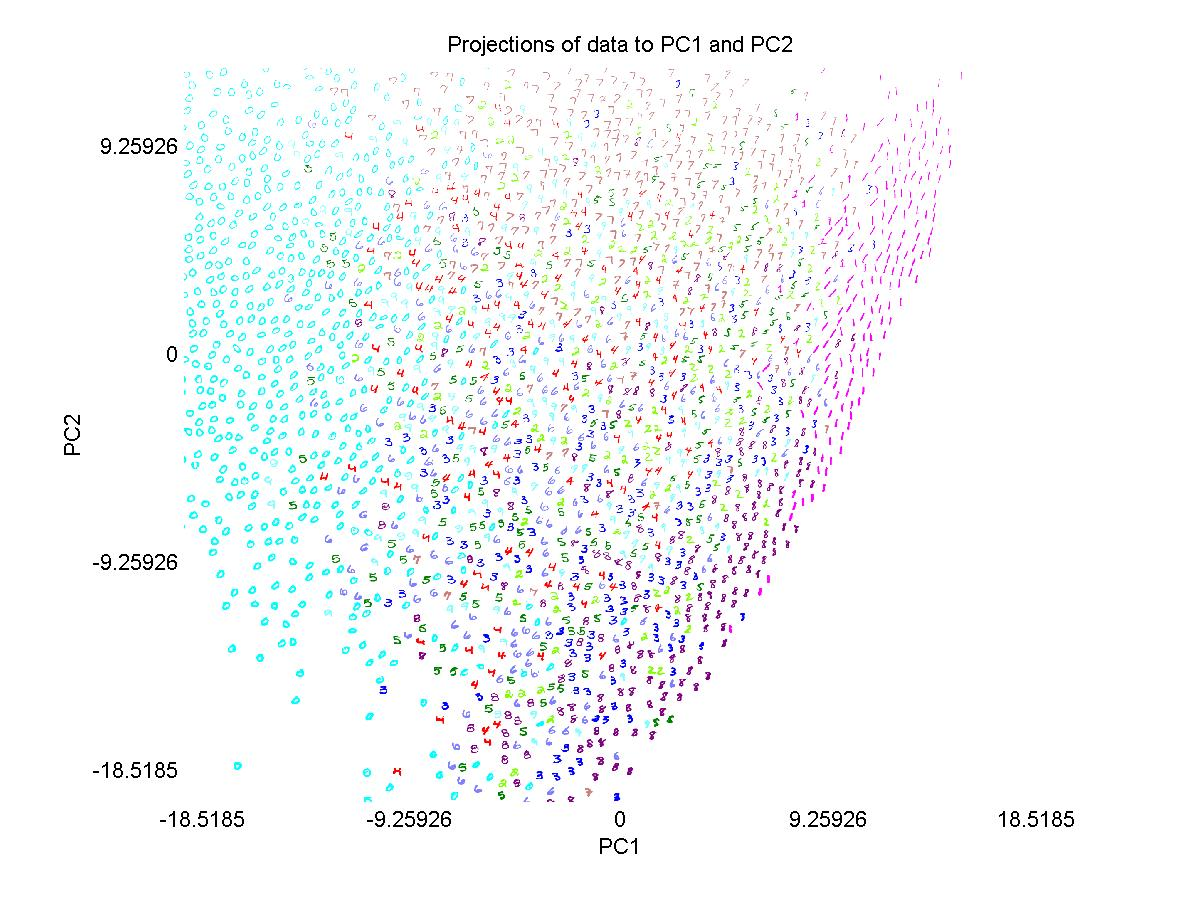
\includegraphics[width=\linewidth]{pc_projections}
\caption{Equal amount of samples from each class was sampled, $N=500$, and then drawn at random if and only if no other digit had been printed at the location in the map. \label{fig:pc_projections}}
\end{figure}
  
One should keep in mind that only the median and 25, 75 percentiles are illustrated and there will be some of the data overlapping. This was also why scatter plots haven’t been used, because a decision about how many samples to plot was needed. Too many would lead to a chaotic plot where some samples disappear behind others and too few do not illustrate the spread well enough. Therefore computing summery statistics over the hole dataset and showing the properties where preferred. It was also experimented with showing mean and confident value given by three times the standard deviation for the distributions instead of the median.

For the PCA the dataset was standardized to mean 0 and unit standard deviation as this generated more intuitive results to interpretive as humans. A machine learning algorithm should be able to solve it either way if the data had only been normalized to zero mean. 
\section{Conclusion}
%Summarize that we have included all the relevant information from the questions raised in the assignment text and tell how good a job we have done.